\documentclass[14pt]{beamer}
\usepackage{./Estilos/BeamerUVM}
\usepackage{./Estilos/ColoresLatex}
\usepackage{circuitikz}
%Sección para el tema de beamer, con el theme, usercolortheme y sección de footers
\usetheme{CambridgeUS}
\usecolortheme{wolverine}
%\useoutertheme{default}
\setbeamercovered{invisible}
% or whatever (possibly just delete it)
\setbeamertemplate{section in toc}[sections numbered]
\setbeamertemplate{subsection in toc}[subsections numbered]
\setbeamertemplate{subsection in toc}{\leavevmode\leftskip=3.2em\rlap{\hskip-2em\inserttocsectionnumber.\inserttocsubsectionnumber}\inserttocsubsection\par}
%\setbeamercolor{section in toc}{fg=blue}
%\setbeamercolor{subsection in toc}{fg=blue}
%\setbeamercolor{frametitle}{fg=blue}
\setbeamertemplate{caption}[numbered]

\setbeamertemplate{footline}
\beamertemplatenavigationsymbolsempty
\setbeamertemplate{headline}{}


\makeatletter
\setbeamercolor{secºtion in foot}{bg=gray!30, fg=black!90!orange}
\setbeamercolor{subsection in foot}{bg=blue!30!yellow, fg=red}
\setbeamercolor{date in foot}{bg=black, fg=white}
\setbeamertemplate{footline}
{
  \leavevmode%
  \hbox{%
  \begin{beamercolorbox}[wd=.333333\paperwidth,ht=2.25ex,dp=1ex,center]{section in foot}%
    \usebeamerfont{section in foot} \insertsection
  \end{beamercolorbox}%
  \begin{beamercolorbox}[wd=.333333\paperwidth,ht=2.25ex,dp=1ex,center]{subsection in foot}%
    \usebeamerfont{subsection in foot}  \insertsubsection
  \end{beamercolorbox}%
  \begin{beamercolorbox}[wd=.333333\paperwidth,ht=2.25ex,dp=1ex,right]{date in head/foot}%
    \usebeamerfont{date in head/foot} \insertshortdate{} \hspace*{2em}
    \insertframenumber{} / \inserttotalframenumber \hspace*{2ex} 
  \end{beamercolorbox}}%
  \vskip0pt%
}






% \usefonttheme{serif}
\usepackage[clock]{ifsym}
\DeclareSIUnit\erg{erg}
\DeclareSIUnit[number-unit-product = {\,}]\cal{cal}

\sisetup{per-mode=symbol}
\resetcounteronoverlays{saveenumi}

% Macro para agregar el logo de UVM en cada slide de la presentación

\addtobeamertemplate{frametitle}{}{%
\begin{tikzpicture}[remember picture,overlay]
\coordinate (logo) at ([xshift=-1.5cm,yshift=-0.8cm]current page.north east);
% \fill[devryblue] (logo) circle (.9cm);
% \clip (logo) circle (.75cm);
\node at (logo) {
\includegraphics[width=2.1cm]{Imagenes/logo_UVM.png}};
\end{tikzpicture}}


\title{\Large{Circuitos eléctricos} \\ \normalsize{Física IV (Área II)}}
\date{}

\begin{document}
\maketitle

\section*{Contenido}
\frame[allowframebreaks]{\frametitle{Contenido} \tableofcontents[currentsection, hideallsubsections]}

\section{Circuitos eléctricos}
\frame{\tableofcontents[currentsection, hideothersubsections]}
\subsection{Definición}

\begin{frame}
\frametitle{¿Qué es un circuito eléctrico?}
Los circuitos eléctricos son sistemas que permiten la circulación de corriente eléctrica para realizar diversas funciones, \pause como proporcionar energía, realizar tareas específicas o transmitir información.
\end{frame}
\begin{frame}
\frametitle{¿Qué es un circuito eléctrico?}
Un circuito eléctrico típico consta de varios componentes interconectados, \pause y la teoría de circuitos eléctricos se basa en principios fundamentales que describen cómo interactúan estos componentes.
\end{frame}

\subsection{Componentes}

\begin{frame}
\frametitle{Fuente de Alimentación}
Proporciona la energía eléctrica al circuito.
\\
\bigskip
\pause
Puede ser una batería, un generador o cualquier dispositivo que suministre voltaje.
\end{frame}
\begin{frame}
\frametitle{Cables o Conductores}
Permiten que la corriente eléctrica fluya desde la fuente de alimentación hasta los dispositivos y componentes del circuito.
\end{frame}
\begin{frame}
\frametitle{Cables o Conductores}    
Los cables están hechos de materiales conductores como el cobre.
\end{frame}
\begin{frame}
\frametitle{Interruptor}
Abre o cierra el circuito, permitiendo o deteniendo el flujo de corriente.
\end{frame}
\begin{frame}
\frametitle{Interruptor}
Es un dispositivo de control que puede estar en posición abierta (apagado) o cerrada (encendido).
\end{frame}
\begin{frame}
\frametitle{Resistencia}
Limita el flujo de corriente en el circuito.
\\
\bigskip
\pause
Se mide en Ohms $(\Omega)$ y se representa con el símbolo $R$.
\end{frame}
\begin{frame}
\frametitle{Capacitor}
Almacena carga eléctrica y libera esa carga cuando sea necesario.
\\
\bigskip
\pause
Su unidad es el Farad $(F)$ y se representa con el símbolo $C$.
\end{frame}
\begin{frame}
\frametitle{Bobina o Inductor}
Almacena energía en forma de campo magnético cuando la corriente fluye a través de ella.
\end{frame}
\begin{frame}
\frametitle{Bobina o Inductor}
Se mide en Henry $(H)$ y se representa con el símbolo $L$.
\end{frame}
\begin{frame}
\frametitle{Diodo}
Permite el flujo de corriente en una dirección \pause y bloquea en la dirección opuesta.
\\
\bigskip
\pause
Se utiliza para rectificación, entre otros propósitos.
\end{frame}

\subsection{Tipos de circuitos}

\begin{frame}
\frametitle{Circuitos en serie}
Los componentes están conectados en una única trayectoria, \pause la corriente tiene que pasar a través de cada componente.
\end{frame}
\begin{frame}
\frametitle{Circuito en serie}
\begin{figure}
\centering
\begin{circuitikz}
 \draw (0,0) to[R=$R_{1}$] (2,0) to[R=$R_{2}$] (4,0) to[R=$R_{3}$] (6,0);
 \draw (0,0)--(0,-2) to[battery1={9 V}] (6,-2)--(6,0);
\end{circuitikz}
\end{figure}
\end{frame}
\begin{frame}
\frametitle{La corriente en un circuito serie}
Como se mencionó, la corriente en el circuito serie es la misma en todos los elementos que lo componen.
\pause
\begin{align*}
I_{T} = I_{1} = I_{2} = I_{3} = \ldots
\end{align*}
\end{frame}
\begin{frame}
\frametitle{El voltaje en un circuito serie}
El voltaje total se \enquote{divide} en cada componente del circuito, es decir:
\pause
\begin{align*}
V_{T} = V_{1} + V_{2} + V_{3} + \ldots 
\end{align*}
\end{frame}
\begin{frame}
\frametitle{La resistencia total}
En un circuito en serie, la resistencia total es:
\pause
\begin{align*}
R_{T} = R_{1} + R_{2} + R_{3} + \ldots
\end{align*}
\end{frame}
\begin{frame}
\frametitle{Circuitos en paralelo}
Los componentes están conectados en múltiples trayectorias, \pause y la corriente se divide entre ellos.
\end{frame}
\begin{frame}
\frametitle{Circuito en paralelo}
\vspace*{-1cm}
\begin{figure}
\centering
\begin{circuitikz}[scale=0.9]
    \draw (0,0) to[R=$R_{1}$] (2,0);
    \draw (0,-2) to[R=$R_{2}$] (2,-2);
    \draw (0,-4)  to[R=$R_{3}$] (2,-4);
    \draw (0,0)--(0,-6) (2,0)--(2,-6);
    \draw (0,-6) to[battery1={9 V}] (2,-6);
   \end{circuitikz}
\end{figure}
\end{frame}
\begin{frame}
\frametitle{La resistencia total}
En el circuito en paralelo, la resistencia total es:
\pause
\begin{align*}
\dfrac{1}{R_{T}} = \dfrac{1}{R_{1}} + \dfrac{1}{R_{2}} + \dfrac{1}{R_{3}} + \ldots
\end{align*}
\end{frame}
\begin{frame}
\frametitle{El voltaje en un circuito en paralelo}
En un circuito en paralelo, el voltaje es el mismo en cada componente:
\pause
\begin{align*}
V_{T} = V_{1} = V_{2} = V_{3} = \ldots
\end{align*}
\end{frame}
\begin{frame}
\frametitle{La corriente en un circuito paralelo}
La corriente en el circuito paralelo se \enquote{divide} en todos los elementos que lo componen.
\end{frame}
\begin{frame}
\frametitle{El corriente en un circuito paralelo}
La corriente total se \enquote{divide} en cada componente del circuito, es decir:
\pause
\begin{align*}
I_{T} = I_{1} + I_{2} + I_{3} + \ldots 
\end{align*}
\end{frame}

\subsection{Circuito mixto}

\begin{frame}
\frametitle{Circuitos mixtos}
Contienen combinaciones de circuitos en serie y en paralelo.
\end{frame}
\begin{frame}
\frametitle{Circuito mixto}
\vspace*{-1cm}
\begin{figure}
\centering
\begin{circuitikz}
\draw (0,0) to[battery1={9 V}]    (0,4) % La fuente de voltaje
            to[R=$R_{1}$] (4,4)
            to[R=$R_{2}$]  (4,0) % La resistencia
            to[short]       (3,0)
            to[short]       (3,.5)
            to [R, a=$R_{3}$] (1,.5)  |-  (0,0) % <---
        (3,0) to[short]       (3,-.5)
            to [R=$R_{4}$] (1,-.5)             % <----
            to [short]      (1,0);
    \end{circuitikz}
\end{figure}
\end{frame}
\begin{frame}
\frametitle{¿Cómo se resuelve?}
Para obtener la resistencia total:
\setbeamercolor{item projected}{bg=lava,fg=white}
\setbeamertemplate{enumerate items}{%
\usebeamercolor[bg]{item projected}%
\raisebox{1.5pt}{\colorbox{bg}{\color{fg}\footnotesize\insertenumlabel}}%
}
\begin{enumerate}[<+->]
\item Se resuelven primero aquellas partes del circuito que estén conectadas en paralelo.
\item Se anota como una resistencia equivalente, con un subíndice: $R_{E1}$.
\seti
\end{enumerate}
\end{frame}
\begin{frame}
\frametitle{Circuito mixto}
\vspace*{-1cm}
\begin{figure}
\centering
\begin{circuitikz}
\draw (0,0) to[battery1={9 V}]    (0,4) % La fuente de voltaje
            to[R=$R_{1}$] (4,4)
            to[R=$R_{2}$]  (4,0) % La resistencia
            to[short]       (3,0)
            % to[short]       (3,.5)
            to [R, a=$R_{E1}$] (1, 0)  |-  (0,0) % <---
            to [short]      (1, 0);
    \end{circuitikz}
\end{figure}
\end{frame}
\begin{frame}
\frametitle{¿Cómo se resuelve?}
\setbeamercolor{item projected}{bg=lava,fg=white}
\setbeamertemplate{enumerate items}{%
\usebeamercolor[bg]{item projected}%
\raisebox{1.5pt}{\colorbox{bg}{\color{fg}\footnotesize\insertenumlabel}}%
}
\begin{enumerate}[<+->]
\conti
\item Buscando dejar un circuito ya sea en serie, o en paralelo, representando una sola resistencia: la resistencia total $R_{T}$
\seti
\end{enumerate}
\end{frame}
\begin{frame}
\frametitle{Circuito mixto}
\vspace*{-1cm}
\begin{figure}
\centering
\begin{circuitikz}
\draw (0, 0) to[battery1={9 V}]    (0, 3) % La fuente de voltaje
            % to[R=$R_{1}$] (4,4)
            to[short]      (3, 3)
            to[R=$R_{T}$]  (3, 0) % La resistencia
            % to[short]       (3,.5)
            % to [R, a=$R_{E1}$] (1, 0)  |-  (0,0) % <---
            to [short]      (0, 0);
    \end{circuitikz}
\end{figure}
\end{frame}
\begin{frame}
\frametitle{¿Cómo se resuelve?}
\setbeamercolor{item projected}{bg=lava,fg=white}
\setbeamertemplate{enumerate items}{%
\usebeamercolor[bg]{item projected}%
\raisebox{1.5pt}{\colorbox{bg}{\color{fg}\footnotesize\insertenumlabel}}%
}
\begin{enumerate}[<+->]
\conti
\item Una vez conocida la resistencia total $(R_{T})$, por la ley de Ohm, se conocerá la corriente total $(I_{T})$
\seti
\end{enumerate}
\end{frame}
\begin{frame}
\frametitle{¿Cómo se resuelve?}
\setbeamercolor{item projected}{bg=lava,fg=white}
\setbeamertemplate{enumerate items}{%
\usebeamercolor[bg]{item projected}%
\raisebox{1.5pt}{\colorbox{bg}{\color{fg}\footnotesize\insertenumlabel}}%
}
\begin{enumerate}[<+->]
\conti
\item Se procede a calcular la corriente y voltaje de cada componente de manera inversa a como se resolvió el circuito.
\end{enumerate}
\end{frame}
\begin{frame}
\frametitle{Resolviendo un ejercicio}
Veamos el procedimiento para calcular el voltaje y la corriente que circula por cada una de las resistencias del siguiente circuito mixto.
\\
\bigskip
\pause
Todas las resistencias valen \SI{10}{\ohm}
\end{frame}
\begin{frame}[plain]
\begin{figure}
\centering
\begin{circuitikz}
    \draw (0, 0) to[battery1={10 V}] (0, 4) % La fuente de voltaje
        to[R=$R_{1}$] (4, 4)
        to[short] (4, 3.5)
        to[short] (3.5, 3.5) |- (4.5, 3.5)
        to[short] (4.5, 3)
        to[R=$R_{3}$] (4.5, 1)
        to[R=$R_{4}$] (4.5, -1)
        to[short] (4, -1)
        to[short] (4, -2)
        to[short] (3, -2)
        to[short] (3, -2.5) |- (3, -1.5)
        to[R, l_=$R_{5}$] (1, -1.5)
        to[short] (1, -2) -- (0, -2) -- (0, 0);
    
    \draw (1, -2) to[short] (1, -2.5)
        to[R, l_=$R_{6}$] (3, -2.5);
    
    \draw (3.5, 3.5) to[R, l_=$R_{2}$] (3.5, -1) -- (4, -1);
\end{circuitikz}
\end{figure}    
\end{frame}
\begin{frame}
\frametitle{Comenzando a simplificar}
Nos fijamos en las resistencias $R_{3}$ y $R_{4}$ que están conectadas en serie.
\\
\bigskip
\pause
La suma de esas resistencias será la resistencia equivalente $R_{E1}$.
\end{frame}
\begin{frame}[plain]
\begin{figure}
\centering
\begin{circuitikz}
    \draw (0, 0) to[battery1={10 V}] (0, 4) % La fuente de voltaje
        to[R=$R_{1}$] (4, 4)
        to[short] (4, 3.5)
        to[short] (3.5, 3.5) |- (4.5, 3.5)
        to[short] (4.5, 3)
        to[R=$R_{3}$] (4.5, 1)
        to[R=$R_{4}$] (4.5, -1)
        to[short] (4, -1)
        to[short] (4, -2)
        to[short] (3, -2)
        to[short] (3, -2.5) |- (3, -1.5)
        to[R, l_=$R_{5}$] (1, -1.5)
        to[short] (1, -2) -- (0, -2) -- (0, 0);
    
    \draw (1, -2) to[short] (1, -2.5)
        to[R, l_=$R_{6}$] (3, -2.5);
    
    \draw (3.5, 3.5) to[R, l_=$R_{2}$] (3.5, -1) -- (4, -1);

    \draw [red, thick] (4.2, 3.25) rectangle (4.8, -1.25);
\end{circuitikz}
\end{figure}    
\end{frame}
\begin{frame}
\frametitle{La resistencia equivalente}
Al estar $R_{3}$ y $R_{4}$ en serie, la resistencia equivalente es:
\pause
\begin{align*}
R_{E1} = R_{1} + R_{2} = \SI{10}{\ohm} + \SI{10}{\ohm} = \SI{20}{\ohm}
\end{align*}
\end{frame}
\begin{frame}
\frametitle{Segunda resistencia equivalente}
Ahora tenemos que $R_{2}$ y $R_{E1}$ están en paralelo, por lo que procedemos a calcular la resistencia equivalente $R_{E2}$
\end{frame}
\begin{frame}[plain]
\begin{figure}
\centering
\begin{circuitikz}
    \draw (0, 0) to[battery1={10 V}] (0, 4) % La fuente de voltaje
        to[R=$R_{1}$] (4, 4)
        to[short] (4, 3.5)
        to[short] (3.5, 3.5) |- (4.5, 3.5)
        to[short] (4.5, 3)
        to[R=$R_{E1}$] (4.5, -1)
        % to[R=$R_{4}$] (4.5, -1)
        to[short] (4, -1)
        to[short] (4, -2)
        to[short] (3, -2)
        to[short] (3, -2.5) |- (3, -1.5)
        to[R, l_=$R_{5}$] (1, -1.5)
        to[short] (1, -2) -- (0, -2) -- (0, 0);
    
    \draw (1, -2) to[short] (1, -2.5)
        to[R, l_=$R_{6}$] (3, -2.5);
    
    \draw (3.5, 3.5) to[R, l_=$R_{2}$] (3.5, -1) -- (4, -1);

    \draw [red, thick] (3.2, 3.75) rectangle (4.8, -1.25);
\end{circuitikz}
\end{figure}    
\end{frame}
\begin{frame}
\frametitle{La resistencia equivalente $R_{E2}$}
\vspace*{-1cm}
Como $R_{2}$ y $R_{E1}$ están en paralelo, la resistencia equivalente $R_{E2}$ es:
\pause
\begin{eqnarray*}
\begin{aligned}
\dfrac{1}{R_{E2}} &= \dfrac{1}{R_{2}} + \dfrac{1}{R_{E1}} \\[0.1em] \pause
R_{E2} &= \dfrac{1}{\dfrac{1}{R_{2}} + \dfrac{1}{R_{E1}}} = \pause \dfrac{1}{\dfrac{1}{\SI{10}{\ohm}} + \dfrac{1}{\SI{20}{\ohm}}} = \pause \dfrac{1}{\dfrac{3}{20} \si{\ohm}} = \\[1em] \pause
R_{E2} &= \SI{6.66}{\ohm}
\end{aligned}
\end{eqnarray*}
\end{frame}
\begin{frame}[plain]
    \begin{figure}
    \centering
    \begin{circuitikz}
    \draw (0, 0) to[battery1={10 V}] (0, 4) % La fuente de voltaje
        to[R=$R_{1}$] (4, 4)
        % to[short] (4, 3.5)
        % to[short] (3.5, 3.5) |- (4.5, 3.5)
        to[short] (4, 3)
        to[R=$R_{E2}$] (4, -1)
        % to[R=$R_{4}$] (4.5, -1)
        to[short] (4, -1)
        to[short] (4, -2)
        to[short] (3, -2)
        to[short] (3, -2.5) |- (3, -1.5)
        to[R, l_=$R_{5}$] (1, -1.5)
        to[short] (1, -2) -- (0, -2) -- (0, 0);
    
    \draw (1, -2) to[short] (1, -2.5)
        to[R, l_=$R_{6}$] (3, -2.5);
    
    % \draw (3.5, 3.5) to[R, l_=$R_{2}$] (3.5, -1) -- (4, -1);

    % \draw [red, thick] (3.2, 3.75) rectangle (4.8, -1.25);
\end{circuitikz}
\end{figure}    
\end{frame}
\begin{frame}
\frametitle{La siguiente resistencia equivalente}
Ahora tenemos en el circuito las resistencias $R_{5}$ y $R_{6}$ en paralelo, al resolverlas, tendremos la resistencia equivalente $R_{E3}$.
\end{frame}
\begin{frame}
\frametitle{Encontrando $R_{3}$}
\begin{eqnarray*}
\begin{aligned}
\dfrac{1}{R_{E3}} &= \dfrac{1}{R_{5}} + \dfrac{1}{R_{6}} \\[1em] \pause
R_{E3} &= \dfrac{1}{\dfrac{1}{R_{5}} + \dfrac{1}{R_{6}}} = \pause \dfrac{1}{\dfrac{1}{\SI{10}{\ohm}} + \dfrac{1}{\SI{10}{\ohm}}} = \pause \dfrac{1}{\dfrac{1}{5} \si{\ohm}} \\[1em] \pause
R_{E3} &= \SI{5}{\ohm}
\end{aligned}
\end{eqnarray*}
\end{frame}
\begin{frame}[plain]
\begin{figure}
\centering
\begin{circuitikz}
\draw (0, 0) to[battery1={10 V}] (0, 4) % La fuente de voltaje
    to[R=$R_{1}$] (4, 4)
    % to[short] (4, 3.5)
    % to[short] (3.5, 3.5) |- (4.5, 3.5)
    to[short] (4, 3)
    to[R=$R_{E2}$] (4, -1)
    % to[R=$R_{4}$] (4.5, -1)
    to[short] (4, -1)
    to[short] (4, -2)
    to[short] (3, -2)
    % to[short] (3, -2.5) |- (3, -1.5)
    to[R, l_=$R_{E3}$] (1, -2)
    to[short] (0, -2) -- (0, 0) ;

% \draw (1, -2) to[short] (1, -2.5)
%     to[R, l_=$R_{6}$] (3, -2.5);

% \draw (3.5, 3.5) to[R, l_=$R_{2}$] (3.5, -1) -- (4, -1);

% \draw [red, thick] (3.2, 3.75) rectangle (4.8, -1.25);
\end{circuitikz}
\end{figure}    
\end{frame}
\begin{frame}
\frametitle{Resistencia total}
Hemos llegado a tres resistencias conectadas en serie, que al resolverlas, tendremos la resistencia total del circuito $R_{T}$.
\end{frame}
\begin{frame}
\frametitle{Resistencia total}
\begin{figure}
\centering
\begin{circuitikz}
\draw (0, 0) to[battery1={10 V}] (0, 4) % La fuente de voltaje
    to[short] (3, 4)
    to[R=$R_{T}$] (3, 0) -- (0, 0);
\end{circuitikz}
\end{figure}    
\end{frame}

\begin{frame}
\frametitle{Resistencia total}
\begin{align*}
R_{T} &= R_{1} + R_{E2} + R_{E3} = \\[1em]
R_{T} &= \SI{10}{\ohm} + \SI{6.6}{\ohm} + \SI{5}{\ohm} = \\[0.5em]
R_{T} &= \SI{21.6}{\ohm}
\end{align*}
\end{frame}
\begin{frame}
\frametitle{Siguiente paso}
Ocupamos la ley de Ohm para resolver la corriente en la resistencia total:
\pause
\begin{align*}
I_{T} = \dfrac{V}{R_{T}} = \dfrac{\SI{10}{\volt}}{\SI{21.6}{\ohm}} = \SI{0.462}{\ampere}
\end{align*}
\end{frame}
\begin{frame}
\frametitle{Calculando valores en las resistencias}
El procedimiento a seguir será de manera inversa y considerando la configuración que tengamos, \pause es decir, \pause ahora vemos el circuito con tres resistencias en serie:
\end{frame}
\begin{frame}[plain]
\begin{figure}
\centering
\begin{circuitikz}
\draw (0, 0) to[battery1={10 V}] (0, 4) % La fuente de voltaje
    to[R=$R_{1}$] (4, 4)
    to[short] (4, 3)
    to[R=$R_{E2}$] (4, -1)
    to[short] (4, -1)
    to[short] (4, -2)
    to[short] (3, -2)
    to[R, l_=$R_{E3}$] (1, -2)
    to[short] (0, -2) -- (0, 0) ;
\end{circuitikz}
\end{figure}    
\end{frame}
\begin{frame}
\frametitle{Valor de voltaje}
Sabemos que en un circuito en serie con tres resistencias:
\pause
\begin{align*}
V_{T} &= V_{1} + V_{E2} + V_{E3} \\[1em]
I_{T} &= I_{1} = I_{E1} = I_{E2}
\end{align*}
\end{frame}
\begin{frame}
\frametitle{Valores de corriente}
\begin{table}[H]
\centering
\begin{tabular}{c | c }
Resistencia & Corriente \\ \hline
$R_{1}$ & \SI{0.462}{\ampere} \\ \hline
$R_{E1}$ & \SI{0.462}{\ampere} \\ \hline
$R_{E2}$ & \SI{0.462}{\ampere} \\ \hline
\end{tabular}
\end{table}
\end{frame}
\begin{frame}
\frametitle{Valores de voltaje}
Con la ley de Ohm, calculamos el valor de voltaje para cada una de estas resistencias:
\end{frame}
\begin{frame}
\frametitle{Valores de voltaje}
\begin{table}[H]
\centering
\begin{tabular}{c | c | c}
Resistencia & Expresión & Voltaje \\ \hline
$R_{1}$ & $V_{1} = (\SI{0.462}{\ampere})(\SI{10}{\ohm})$ & \SI{4.62}{\volt} \\ \hline
$R_{E2}$ & $V_{E2} = (\SI{0.462}{\ampere})(\SI{6.6}{\ohm})$ & \SI{3.049}{\volt} \\ \hline
$R_{E3}$ & $V_{E3} = (\SI{0.462}{\ampere})(\SI{5}{\ohm})$ & \SI{2.31}{\volt} \\ \hline
\end{tabular}
\end{table}    
\end{frame}
\begin{frame}
\frametitle{Resolviendo $R_{E2}$}
Como ya se tiene el voltaje de la resistencia equivalente $R_{E2}$, \pause podemos obtener los valores de corriente y voltaje de las resistencias $R_{2}$ y $R_{E1}$ que están en paralelo.
\pause
\begin{align*}
V_{E2} = V_{2} = V_{E1}
\end{align*}
\end{frame}
\begin{frame}
\frametitle{Valores de voltaje}
\begin{table}[H]
\centering
\begin{tabular}{c | c }
Resistencia & Voltaje \\ \hline
$R_{2}$ & $V_{2} = \SI{3.049}{\volt}$ \\ \hline
$R_{E1}$ & $V_{E1} = \SI{3.049}{\volt}$ \\ \hline
\end{tabular}
\end{table}    
\end{frame}
\begin{frame}
\frametitle{Valores de corriente}
Obtenemos la corriente usando la ley de Ohm:
\begin{table}[H]
\centering
\begin{tabular}{c | c | c}
Resistencia & Expresión & Corriente \\ \hline
$R_{2}$ & $I_{2} = \dfrac{\SI{3.049}{\volt}}{\SI{10}{\ohm}}$ & \SI{0.304}{\ampere} \\ \hline
$R_{E1}$ & $I_{E1} = \dfrac{\SI{3.049}{\volt}}{\SI{6.6}{\ohm}}$ & \SI{0.1524}{\ampere} \\ \hline
\end{tabular}
\end{table}    
\end{frame}
\begin{frame}
\frametitle{Resolviendo $R_{E1}$}
La resistencia $R_{E1}$ corresponde a las resistencias en serie $R_{3}$ y $R_{4}$, por lo que posible obtener sus valores de corriente y voltaje.
\end{frame}
\begin{frame}
\frametitle{Valores de corriente}
\vspace*{-1cm}
\[ I_{E1} = I_{3} = I_{4} \]
\begin{table}[H]
\centering
\begin{tabular}{c | c }
Resistencia & Corriente \\ \hline
$R_{3}$ & $I_{3} = \SI{0.4619}{\ampere}$ \\ \hline
$R_{4}$ & $I_{4} = \SI{0.4619}{\ampere}$ \\ \hline
\end{tabular}
\end{table}    
\end{frame}
\begin{frame}
\frametitle{Valores de voltaje}
\begin{table}[H]
\centering
\begin{tabular}{c | c | c}
Resistencia & Expresión & Voltaje \\ \hline
$R_{3}$ & $V_{3} = (\SI{0.1524}{\ampere})(\SI{10}{\ohm})$ & \SI{01.524}{\volt} \\ \hline
$R_{4}$ & $V_{4} = (\SI{0.1524}{\ampere})(\SI{10}{\ohm})$ & \SI{01.524}{\volt} \\ \hline
\end{tabular}
\end{table}    
\end{frame}
\begin{frame}
\frametitle{Valores en $R_{E3}$}
Nos resta calcular los valores de corriente y voltaje en $R_{E3}$, que la conforman las resistencias $R_{5}$ y $R_{6}$ conectadas en paralelo.
\end{frame}
\begin{frame}
\frametitle{Valores de voltaje}
\vspace*{-1cm}
\[ V_{E3} = V_{5} = V_{6} \]
\begin{table}[H]
\centering
\begin{tabular}{c | c }
Resistencia & Corriente \\ \hline
$R_{5}$ & $V_{5} = \SI{2.31}{\volt}$ \\ \hline
$R_{6}$ & $V_{6} = \SI{2.31}{\volt}$ \\ \hline
\end{tabular}
\end{table}    
\end{frame}
\begin{frame}
\frametitle{Valores de corriente}
Obtenemos la corriente usando la ley de Ohm:
\begin{table}[H]
\centering
\begin{tabular}{c | c | c}
Resistencia & Expresión & Corriente \\ \hline
$R_{5}$ & $I_{5} = \dfrac{\SI{2.31}{\volt}}{\SI{10}{\ohm}}$ & \SI{0.231}{\ampere} \\ \hline
$R_{6}$ & $I_{6} = \dfrac{\SI{2.31}{\volt}}{\SI{10}{\ohm}}$ & \SI{0.231}{\ampere} \\ \hline
\end{tabular}
\end{table}    
\end{frame}
\begin{frame}
\frametitle{Trabajo completo}
Ya se han calculado las corrientes y voltajes en cada una de las resistencias del circuito mixto, se aconseja presentar una tabla con los valores.
\end{frame}
\begin{frame}
\frametitle{Valores para las resistencias}
\begin{table}[H]
\centering
\renewcommand{\arraystretch}{0.8}
\begin{tabular}{| c | c | c |} \hline
Resistencia & Voltaje & Corriente \\ \hline
$R_{1}$ & \SI{4.620}{\volt} & \SI{0.462}{\ampere} \\ \hline
$R_{2}$ & \SI{3.049}{\volt} & \SI{0.304}{\ampere} \\ \hline
$R_{3}$ & \SI{1.524}{\volt} & \SI{0.1524}{\ampere} \\ \hline
$R_{4}$ & \SI{1.524}{\volt} & \SI{0.1524}{\ampere} \\ \hline
$R_{5}$ & \SI{2.31}{\volt} & \SI{0.231}{\ampere} \\ \hline
$R_{6}$ & \SI{2.31}{\volt} & \SI{0.231}{\ampere} \\ \hline
\end{tabular}
\end{table}
\end{frame}

\section{Reactancias}
\frame{\tableofcontents[currentsection, hideothersubsections]}

\subsection{Reactancia capacitiva}

\begin{frame}
\frametitle{¿Qué es la reactancia capacitiva?}
La \textocolor{darkblue}{reactancia capacitiva} es la oposición que presenta un capacitor al paso de la corriente.
\end{frame}
\begin{frame}
\frametitle{Circuito $R \, C$}
\vspace*{-1cm}
Cuando tenemos un circuito $R \, C$
\begin{center}
\begin{circuitikz}[american voltages]
        \draw
        (0, 0) to[sI] ++(0, 3)
        to[R, l=$R$] ++(4, 0)
        to[C, l=$C$] ++(0, -3)
        to[short] (0, 0);
\end{circuitikz} 
\end{center}
\end{frame}
\begin{frame}
\frametitle{Voltaje en el capacitor}    
En un capacitor para obtener la fórmula del voltaje, \pause se parte de la fórmula de la corriente que es
\pause
\begin{align*}
I_{c \, \text{máx}} = V_{c \, \text{máx}} \cdot \omega \, C
\end{align*}
y se despeja para obtener la fórmula de voltaje:
\end{frame}
\begin{frame}
\frametitle{La reactancia capacitiva}
\begin{align*}
V_{c \, \text{máx}} = I_{c \, \text{máx}} \left(  \dfrac{1}{\omega \, C} \right)
\end{align*}
\pause
el término en el paréntesis se le conoce como \textocolor{lava}{reactancia capacitiva} $(X_{C})$.
\end{frame}
\begin{frame}
\frametitle{La reactancia capacitiva}
\vspace*{-1cm}
Definimos la reactancia capacitiva como:
\pause
\begin{align*}
X_{C} = \dfrac{1}{\omega \, C}
\end{align*}
Donde:
\setbeamercolor{item projected}{bg=cyan,fg=crimson}
\setbeamertemplate{enumerate items}{%
\usebeamercolor[bg]{item projected}%
\raisebox{1.5pt}{\colorbox{bg}{\color{fg}\footnotesize\insertenumlabel}}%
}
\begin{enumerate}[<+->]
\item $\omega$ es la frecuencia angular de la fuente de alimentación (se mide en \si{\radian\per\second})
\item $C$ es la capacitancia (se mide en Faradios)
\end{enumerate}
\end{frame}
\begin{frame}
\frametitle{La reactancia capacitiva}
La \textocolor{lava}{reactancia capacitiva} $(X_{C})$ se interpreta como la oposición que presenta el capacitor al paso de la corriente, \pause se mide en Ohms (\si{\ohm}).
\end{frame}
\begin{frame}
\frametitle{Manejando la reactancia capacitiva}
La \textocolor{lava}{reactancia capacitiva} $(X_{C})$ es diferente a la \textocolor{copper}{resistencia normal} $(R)$, \pause aunque ambas se miden en Ohms $\si{\ohm}$, no se puede sumar directamente por dos razones:
\end{frame}
\begin{frame}
\frametitle{Manejando la reactancia capacitiva}
\setbeamercolor{item projected}{bg=darklava,fg=white}
\setbeamertemplate{enumerate items}{%
\usebeamercolor[bg]{item projected}%
\raisebox{1.5pt}{\colorbox{bg}{\color{fg}\footnotesize\insertenumlabel}}%
}
\begin{enumerate}[<+->]
\item Aunque provoca que exista una corriente en el circuito, produce un desfasamiento de \ang{90} entre voltaje y corriente.
\item No consume energía.
\end{enumerate}
\end{frame}
\begin{frame}
\frametitle{Relación entre V - I}
\vspace*{-1cm}
La corriente \textocolor{bulgarianrose}{está en fase} con respecto al voltaje.
\begin{figure}
    \centering
    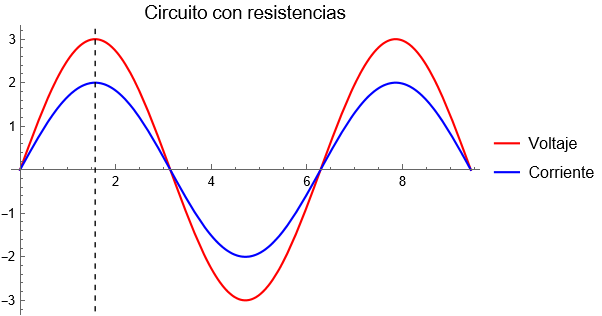
\includegraphics[scale=0.6]{Imagenes/Circuitos_IV_01.png}
\end{figure}
\end{frame}
\begin{frame}
\frametitle{Defasamiento entre V - I}
\vspace*{-1cm}
\textocolor{cobalt}{La corriente se adelanta} \ang{90} con respecto al voltaje.
\begin{figure}
    \centering
    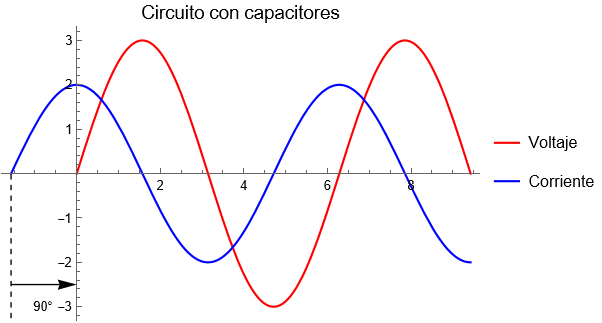
\includegraphics[scale=0.6]{Imagenes/Circuitos_IV_02.png}
\end{figure}
\end{frame}
\begin{frame}
\frametitle{La reactancia capacitiva}
De esta manera, nos referimos a ella como una \textocolor{darkmagenta}{resistencia imaginaria}.
\end{frame}
\begin{frame}
\frametitle{Circuito $R \, C$}
\vspace*{-1cm}
\begin{center}
\begin{circuitikz}[american voltages]
      \draw
       (0, 0) to[sI] ++(0, 3)
        to[R, l=$R$] ++(4, 0)
        to[C, l=$C$] ++(0, -3)
        to[short] (0, 0);
\end{circuitikz} 
\end{center}
La \enquote{resistencia total} del circuito $R \, C$ se llama \textocolor{cardinal}{impedancia eléctrica} $(Z)$, que se mide en Ohms (\si{\ohm}).
\end{frame}
\begin{frame}
\frametitle{Impedancia compleja en un circuito $R \, C$}
La impedancia eléctrica $(Z)$ en el circuito $R \, C$ se representa como un número complejo:
\pause
\begin{align*}
Z = R - j \, X_{C}
\end{align*}
\end{frame}
\begin{frame}
\frametitle{Impedancia compleja en un circuito $R \, C$}
\vspace*{-1cm}
\begin{align*}
Z = R - j \, X_{C}
\end{align*}
Donde:
\setbeamercolor{item projected}{bg=carolinablue,fg=black}
\setbeamertemplate{enumerate items}{%
\usebeamercolor[bg]{item projected}%
\raisebox{1.5pt}{\colorbox{bg}{\color{fg}\footnotesize\insertenumlabel}}%
}
\begin{enumerate}[<+->]
\item $R$ es la parte real.
\item $X_{C}$ es la parte imaginaria.
\item $j = \sqrt{-1}$
\end{enumerate}
\end{frame}
\begin{frame}
\frametitle{El signo en $Z$}
El signo negativo de la parte imaginaria $(- j \, X_{C})$ se debe al defasamiento entre la corriente y el voltaje en el circuito $R \, C$.
\end{frame}
\begin{frame}
\frametitle{Ejercicio}
A un circuito serie RC con $R = \SI{20}{\ohm}$ y $C = \SI{5}{\micro\farad}$, se le aplica un voltaje $V = \num{150} \, \cos (\num{10000}) \, t $\, Volts.
\\
\bigskip
\pause
Calcula la impedancia compleja $Z = R + i \, X_{C}$.
\end{frame}
\begin{frame}
\frametitle{Solución}
\textocolor{red}{Datos:}
\vspace*{-1cm}
\begin{align*}
R &= \SI{20}{\ohm} \\
C &= \SI{5}{\micro\farad} \\
\omega &= \num{10000} \, \text{rad/s} \\
X_{C} &= \,?  \\
Z &= \, ?
\end{align*} 
\end{frame}
\begin{frame}
\frametitle{Solución}
\textocolor{red}{Expresiones:}
\pause
\begin{align*}
X_{C} &= \dfrac{1}{\omega \, C} \\[0.5em]
Z &= R + j \, X_{C}
\end{align*}
\end{frame}
\begin{frame}
\frametitle{Solución}
\textocolor{red}{Sustitución:}
\begin{eqnarray*}
\begin{aligned}
X_{C} &= \dfrac{1}{\omega \, C} = \dfrac{1}{(\num{10000} \, \text{rad/s})\left( \SI{5d-6}{\farad} \right)} \\ \pause
X_{C} &= \SI{20}{\ohm}
\end{aligned}
\end{eqnarray*}
\end{frame}
\begin{frame}
\frametitle{Solución}
Por lo que la impedancia compleja del circuito serie RC es:
\pause
\begin{align*}
Z = 20 - j \, 20
\end{align*}
\end{frame}
\begin{frame}
\frametitle{Magnitud de la impedancia}
Ya sabemos cómo escribir la impedancia compleja de un circuito $RC$, \pause pero podemos obtener el valor de la misma, lo que nos permitiría \enquote{conectar} con otros elementos y obtener una resistencia total.
\end{frame}
\begin{frame}
\frametitle{Magnitud de la Impedancia}
La magnitud de la impedancia en un circuito $RC$, se obtiene de la siguiente manera:
\pause
\begin{align*}
Z = \sqrt{R^{2} + \left( X_{C} \right)^{2}}
\end{align*}
El valor de $Z$ se reporta en Ohms $(\si{\ohm})$.
\end{frame}

\subsection{Reactancia inductiva}

\begin{frame}
\frametitle{Circuito $R \, L$}
\vspace*{-1cm}
Cuando tenemos un circuito $R \, L$
\begin{center}
\begin{circuitikz}[american voltages]
        \draw
        (0, 0) to[sI] ++(0, 3)
        to[R, l=$R$] ++(4, 0)
        to[L, l=$L$] ++(0, -3)
        to[short] (0, 0);
\end{circuitikz} 
\end{center}
\end{frame}
\begin{frame}
\frametitle{¿Qué es la reactancia inductiva?}
La \textocolor{darkscarlet}{reactancia inductiva} es la oposición que presenta un inductor al paso de la corriente.
\end{frame}
\begin{frame}
\frametitle{¿Qué es la reactancia inductiva?}
Tampoco se puede llamar resistencia ya que el inductor también produce un desfasamiento de \ang{90} entre la corriente y el voltaje.
\end{frame}
\begin{frame}
\frametitle{Defasamiento entre V - I}
\vspace*{-1cm}
\textocolor{byzantine}{La corriente se retrasa} \ang{90} con respecto al voltaje.
\begin{figure}
    \centering
    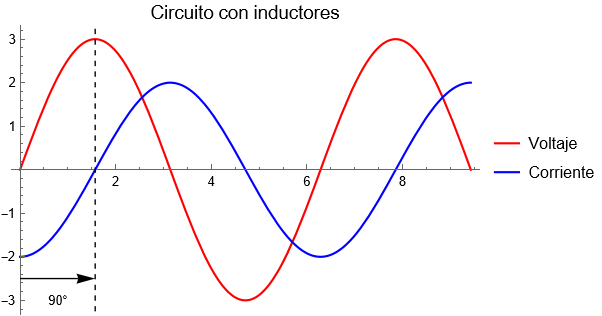
\includegraphics[scale=0.6]{Imagenes/Circuitos_IV_03.png}
\end{figure}
\end{frame}
\begin{frame}
\frametitle{Voltaje en el inductor}
Si la ecuación del inductor
\pause
\begin{align*}
V_{L \, \text{máx}} = I_{L \, \text{máx}} \cdot \omega \cdot L
\end{align*}
\pause 
se analiza como a la Ley de Ohm en las resistencias $(V = I \, R)$,
\end{frame}
\begin{frame}
\frametitle{Voltaje en el inductor}
Quedaría de la siguiente manera para el inductor:
\pause
\begin{align*}
V_{L \, \text{máx}} = I_{L \, \text{máx}} \cdot \left( \omega \cdot L \right)
\end{align*}
\end{frame}
\begin{frame}
\frametitle{Reactancia inductiva}
Al elemento entre paréntesis, se le conoce como \textocolor{darkviolet}{reactancia inductiva}:
\pause
\begin{align*}
X_{L} = \omega \cdot L
\end{align*}
\end{frame}
\begin{frame}
\frametitle{Reactancia inductiva}
\vspace*{-1cm}
\begin{align*}
X_{L} = \omega \cdot L
\end{align*}
Donde:
\setbeamercolor{item projected}{bg=darkslateblue,fg=white}
\setbeamertemplate{enumerate items}{%
\usebeamercolor[bg]{item projected}%
\raisebox{1.5pt}{\colorbox{bg}{\color{fg}\footnotesize\insertenumlabel}}%
}
\begin{enumerate}[<+->]
\item $\omega$ es la frecuencia angular de la fuente de alimentación (se mide en \si{\radian\per\second}).
\item $L$ es la inductancia de la bobina/inductor (se mide en Henry [\si{\henry}]).
\end{enumerate}
\end{frame}
\begin{frame}
\frametitle{Reactancia inductiva}
La \textocolor{ao}{reactancia inductiva} $X_{L}$ es la oposición que presenta el inductor al paso de la corriente a través de él, se mide en Ohms $(\si{\ohm})$.
\end{frame}
\begin{frame}
\frametitle{Manejando la reactancia inductiva}
La \textocolor{ao}{reactancia inductiva} $(X_{L})$ tampoco se puede sumar con la \textocolor{bole}{resistencia} $(R)$, y se trabaja en forma matemática como una resistencia imaginaria.
\end{frame}
\begin{frame}
\frametitle{Impedancia en un circuito $R \, L$}
La \enquote{resistencia total} del circuito $R \, L$ se llama \textocolor{electricindigo}{impedancia eléctrica} $(Z)$, que se mide en Ohms (\si{\ohm}).
\end{frame}
\begin{frame}
\frametitle{Impedancia en un circuito $R \, L$}
La \textocolor{electricindigo}{impedancia compleja} $Z$ en un circuito $R \, L$ se representa como un número complejo:
\pause
\begin{align*}
Z = R + j \, X_{L}
\end{align*}
\end{frame}
\begin{frame}
\frametitle{Impedancia compleja en un circuito $R \, L$}
\vspace*{-1cm}
\begin{align*}
Z = R + j \, X_{L}
\end{align*}
Donde:
\setbeamercolor{item projected}{bg=carolinablue,fg=black}
\setbeamertemplate{enumerate items}{%
\usebeamercolor[bg]{item projected}%
\raisebox{1.5pt}{\colorbox{bg}{\color{fg}\footnotesize\insertenumlabel}}%
}
\begin{enumerate}[<+->]
\item $R$ es la parte real.
\item $X_{L}$ es la parte imaginaria.
\item $j = \sqrt{-1}$
\end{enumerate}
\end{frame}
\begin{frame}
\frametitle{El signo en $Z$}
El signo positivo de la parte imaginaria $(+ j \, X_{L})$ se debe al defasamiento entre la corriente y el voltaje en el circuito $R \, L$.
\end{frame}
\begin{frame}
\frametitle{Magnitud de la Impedancia}
La magnitud de la impedancia en un circuito $RL$, se obtiene de la siguiente manera:
\pause
\begin{align*}
Z = \sqrt{R^{2} + \left( X_{L} \right)^{2}}
\end{align*}
El valor de $Z$ se reporta en Ohms $(\si{\ohm})$.
\end{frame}

\begin{frame}
\frametitle{Manejando las reactancias}
En cambio, la reactancia inductiva y la reactancia capacitiva \textocolor{blue}{sí se pueden sumar entre sí}, \pause ya que ambas son interpretadas matemáticamente como resistencias negativas.
\end{frame}
\begin{frame}
\frametitle{Manejando las reactancias}
En el inductor el voltaje va adelantado \ang{90} a la corriente \pause y en el capacitor el voltaje va retrasado \ang{90} a la corriente.
\end{frame}
\begin{frame}
\frametitle{Manejando las reactancias}
Ambos elementos, al sumarse pueden cancelar sus efectos entre sí y es por eso que sus reactancias imaginarias tienen que ser de signos contrarios.
\end{frame}

\section{Impedancia en \texorpdfstring{$RLC$}{RLC}}
\frame{\tableofcontents[currentsection, hideothersubsections]}
\subsection{La impedancia compleja}

\begin{frame}
\frametitle{Circuito RLC en serie}
\vspace*{-1cm}
Considera el siguiente circuito $RLC$:
\pause
\begin{center}
    \begin{circuitikz}[american voltages]
            \draw
            (0, 0) to [sI] ++(0, 3)
            to [R, l=$R$] ++(4, 0)
            to [L, l=$L$] ++(0, -3)
            to [C, l=$C$] ++(-3, 0)
            to [short] (0, 0);
    \end{circuitikz} 
    \end{center}
\end{frame}
\begin{frame}
\frametitle{La impedancia compleja}
Obtener la impedancia compleja del circuito $RLC$ en serie, es mediante la siguiente expresión:
\pause
\begin{align*}
Z = R + j \, \left( X_{L} - X_{C} \right)
\end{align*}
\end{frame}
\begin{frame}
\frametitle{Magnitud de la impedancia}
La magnitud de la impedancia del circuito $RLC$ en serie, se obtiene de manera similar que para la reactancia capacitiva y la reactancia inductiva:
\end{frame}
\begin{frame}
\frametitle{Magnitud de la impedancia}
Valor de la impedancia eléctrica del circuito $RLC$:
\pause
\begin{align*}
Z = \sqrt{R^{2} + \left( X_{L} - X_{C} \right)^{2}}
\end{align*}
El valor de $Z$ se expresa en Ohms $(\si{\ohm})$.
\end{frame}
\begin{frame}
\frametitle{Resumen}
\begin{table}
    \centering
    \fontsize{12}{12}\selectfont
    \begin{tabular}{c | c | c}
        Elemento & $Z$ compleja & $Z$ Magnitud \\ \hline
        $R \, C$ & $Z = R - j \, X_{C}$ & $Z = \sqrt{R^{2} + \left( X_{C} \right)^{2}}$ \\ \hline
        $R \, L$ & $Z = R + j \, X_{L}$ & $Z = \sqrt{R^{2} + \left( X_{L} \right)^{2}}$ \\ \hline
        $R \, L \, C$ & $Z = R + j \, (X_{L} - X_{C})$ & $Z = \sqrt{R^{2} + \left( X_{L} - X_{C}\right)^{2}}$ \\ \hline
    \end{tabular}
\end{table}
\end{frame}

\section{Ejercicios}
\frame{\tableofcontents[currentsection, hideothersubsections]}
\subsection{Circuito RC}

\begin{frame}
\frametitle{Constante de tiempo}
\vspace*{-1cm}
En un circuito $RC$ en serie:
\pause
\begin{center}
\begin{circuitikz}[american voltages]
        \draw
        (0, 0) to [battery, l=$\SI{40}{\volt}$] ++(0, 3)
        to [R, l^= $\SI{8}{\kilo\ohm}$] ++(4, 0)
        % to [short] ++(1, 0)
        % to [L, l=$L$] ++(0, -3)
        to [C, l=$\SI{4}{\micro\farad}$] ++(0, -3)
        to [short] (0, 0);
\end{circuitikz} 
\end{center}
\end{frame}
\begin{frame}
\frametitle{Constante de tiempo}
\setbeamercolor{item projected}{bg=bananayellow,fg=ao}
\setbeamertemplate{enumerate items}{%
\usebeamercolor[bg]{item projected}%
\raisebox{1.5pt}{\colorbox{bg}{\color{fg}\footnotesize\insertenumlabel}}%
}
\begin{enumerate}[<+->]
\item ¿Cuál es el valor de la constante de tiempo $\tau$?
\item ¿Cuál es la expresión para el voltaje en el ciclo de carga del capacitor?
\end{enumerate}    
\end{frame}
\begin{frame}
\frametitle{Valor de la constante de tiempo}
La constante de tiempo $\tau$ se obtiene:
\pause
\begin{eqnarray*}
\begin{aligned}
\tau &= \pause R \, C = \pause (\SI{8}{\kilo\ohm})(\SI{4}{\micro\farad}) = \\[0.5em] \pause
&= (\SI{8d3}{\ohm})(\SI{4d-6}{\farad}) = \pause \SI{0.032}{\milli\second}
\end{aligned}
\end{eqnarray*}
\end{frame}
\begin{frame}
\frametitle{Expresión para el ciclo de carga}
El voltaje en el ciclo de carga del condensador es:
\pause
\begin{eqnarray*}
\begin{aligned}
V = V_{0} \, \left[ 1 - \exp \left(- \dfrac{t}{\tau} \right) \right] = \\[0.5em] \pause
V = 40 \, \left[ 1 - \exp \left(- \dfrac{t}{\SI{0.032}\second} \right) \right]
\end{aligned}
\end{eqnarray*} 
\end{frame}
\begin{frame}
\frametitle{Gráfica de voltaje capacitor}
\begin{figure}
    \centering
    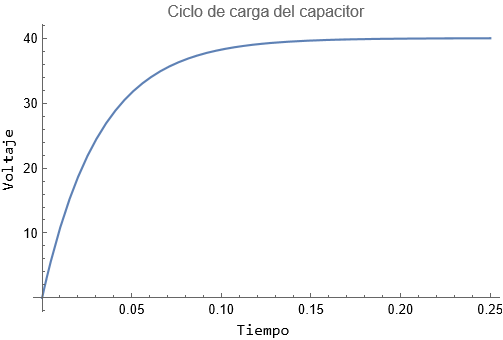
\includegraphics[scale=0.6]{Imagenes/Carga_Capacitor_01.png}
\end{figure}
\end{frame}
\begin{frame}
\frametitle{Valor de voltaje}
Se pregunta: ¿Cuánto tiempo transcurre para que en el capacitor haya un voltaje de \SI{20}{volt}?
\end{frame}
\begin{frame}
\frametitle{Resistencias en serie}
Considera el circuito de resistencias en serie:
\pause 
\begin{center}
\begin{circuitikz}[american voltages]
    \draw 
        (0, 0) node [anchor=east] {$A^{\prime}$}
        to[short, o-] (1, 0)
        % (0, 0) to[V=10V] (0, 4)
        to [R, l=\mbox{$R$}] (3, 0)
        to [R, l=\mbox{$R$}] (5, 0)
        to [R, l=\mbox{$R$}] (7, 0)
        to [R, l=\mbox{$R$}] (9, 0)
        % -- (8.5, 0) node[midway,fill=white,inner sep=5,scale=1.2] {$.\,.\,.$} (10.5, 0)
        % ;
        % \draw (8.5, 0) to [R, l=\mbox{$R$}] (10.5, 0)
            to[short, -o] (10, 0)
            node [anchor=west] {$B^{\prime}$};
\end{circuitikz}  
\end{center}
\pause
¿Cuál es el valor de la resistencia total $R_{T}$?
\end{frame}
\begin{frame}
\frametitle{Resistencias en paralelo}
\vspace*{-1cm}
Considera el circuito de resistencias en paralelo:
\pause
\begin{center}
\begin{circuitikz}[american voltages]
\draw 
    (0, 0) node [anchor=east] {$A^{\prime}$}
    to[short, o-] (2, 0)
    % (0, 0) to[V=10V] (0, 4)
    to [R, l=\mbox{$R$}] (2, -2)
    to [short, -o] (0, -2)
    (-0.75, -2) node [anchor=west]{$B^{\prime}$};
\draw (2, 0) to [short] (4, 0)
    to [R, l=\mbox{$R$}] (4, -2)
    to [short] (2, -2);
\draw (4, 0) to [short] (6, 0)
to [R, l=\mbox{$R$}] (6, -2)
to [short] (4, -2);
\draw (6, 0) to [short] (8, 0)
to [R, l=\mbox{$R$}] (8, -2)
to [short] (6, -2);
% \draw (6, 0) -- (8, 0) node[midway,fill=white,inner sep=5,scale=1.2] {$.\,.\,.$};
% \draw (6, -2) -- (8, -2) node[midway,fill=white,inner sep=5,scale=1.2] {$.\,.\,.$};
\end{circuitikz}  
\end{center}
\pause
\pause
¿Cuál es el valor de la resistencia total $R_{T}$?
\end{frame}

\end{document}